\documentclass[tikz,border=10pt]{standalone}
\usepackage{amsmath}
\usetikzlibrary{arrows.meta, positioning, calc, decorations.pathreplacing}
\definecolor{c1}{HTML}{000000}
\definecolor{c2}{HTML}{233D4D}
\definecolor{c3}{HTML}{FE7F2D}
\definecolor{c4}{HTML}{EAECF0}
\definecolor{labelcolor}{HTML}{5F6B75}
\begin{document}
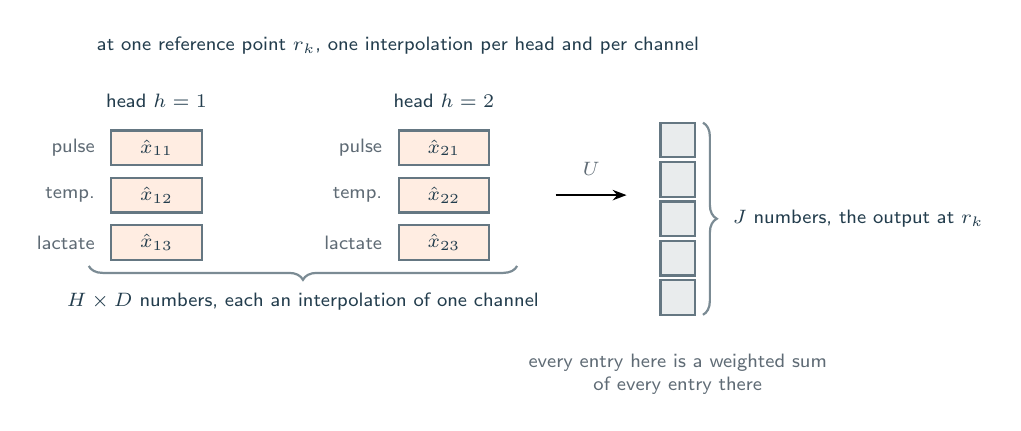
\begin{tikzpicture}[
    every node/.style={font=\sffamily},
    lab/.style={font=\sffamily\scriptsize, text=labelcolor},
    tag/.style={font=\sffamily\scriptsize, text=c2},
    hot/.style={font=\sffamily\scriptsize, text=c3!85!black},
    cell/.style={rectangle, draw=c2!70, fill=c3!14, line width=0.8pt,
                 minimum width=1.15cm, minimum height=0.44cm,
                 font=\sffamily\scriptsize, text=c2, inner sep=1pt},
    ocell/.style={rectangle, draw=c2!70, fill=c2!10, line width=0.8pt,
                minimum width=0.44cm, minimum height=0.44cm},
    arr/.style={-{Stealth[length=5pt]}, line width=1.0pt, color=c1},
]

\node[tag, anchor=west] at (0.60, 5.55)
    {at one reference point $r_k$, one interpolation per head and per channel};

% H = 2 heads, D = 3 channels
\foreach \h/\xo in {1/0.90, 2/4.55}{
    \node[tag] at ({\xo+0.58}, 4.85) {head $h = \h$};
    \foreach \d/\y/\name in {1/4.25/{pulse}, 2/3.65/{temp.}, 3/3.05/{lactate}}{
        \node[cell] at ({\xo+0.58}, \y) {$\hat{x}_{\h\d}$};
        \node[lab, anchor=east] at ({\xo-0.08}, \y) {\name};
    }
}

\draw[decorate, decoration={brace, amplitude=5pt, mirror}, c2!60, line width=0.8pt]
    (0.62, 2.75) -- (6.06, 2.75)
    node[midway, below=6pt, font=\sffamily\scriptsize, text=c2]
    {$H \times D$ numbers, each an interpolation of one channel};

\draw[arr] (6.55, 3.65) -- (7.45, 3.65);
\node[lab, anchor=south, align=center] at (7.00, 3.78) {$U$};

\foreach \j in {0,...,4}{
    \node[ocell] at (8.10, {4.35 - \j*0.50}) {};
}
\draw[decorate, decoration={brace, amplitude=5pt}, c2!60, line width=0.8pt]
    (8.42, 4.57) -- (8.42, 2.13)
    node[midway, right=7pt, font=\sffamily\scriptsize, text=c2]
    {$J$ numbers, the output at $r_k$};

\node[lab, anchor=north, align=center] at (8.10, 1.75)
    {every entry here is a weighted sum\\ of every entry there};
\end{tikzpicture}
\end{document}
